% This file is part of the Open Source project 'proTironeComputatri'
% (c) 2025 Karsten Reincke (https://github.com/kreincke/proTironeComputatri)
% It is distributed under the terms of the creative commons license
% CC-BY-4.0 (= https://creativecommons.org/licenses/by/4.0/)

\documentclass[
  DIV=calc,
  BCOR=5mm,
  11pt,
  headings=small,
  oneside,
  abstract=true,
  toc=bib,
  english,ngerman]{scrartcl}

% customize your presentation
% ---------------------------
% set paths:

\def\imgGl{../../../img.gl/}
\def\bibGl{../../../bib.gl}
\def\cfgGl{../../../cfg.gl/}
\def\imgLf{../../img.lf}
\def\cfgLf{../../cfg.lf}
\def\bibLf{../../bib.lf}

\usepackage[utf8]{inputenc}
\usepackage{a4}
\usepackage[english,ngerman]{babel}

\usepackage[
  backend=biber,
  style=authortitle-dw,
  sortlocale=auto,
]{biblatex}
\input{\cfgGl/inc.cfg-biber-de.tex}

\addbibresource{\bibLf/lit.lf00.bib}

% package for improving the grey value and the line feed handling
\usepackage{microtype}

%language specific quoting signs
\usepackage[style=german,autostyle=true,]{csquotes}

% language specific hyphenation
\input{\cfgGl/inc.babelhyphenations.tex}

%%% (3) layout page configuration %%%

% select the visible parts of a page
% S.31: { plain|empty|headings|myheadings }
\pagestyle{headings}
% select the wished style of page-numbering
% S.32: { arabic,roman,Roman,alph,Alph }
\pagenumbering{arabic}
\setcounter{page}{1}

% select the wished distances using the general setlength order:
% S.34 { baselineskip| parskip | parindent }
% - general no indent for paragraphs
\setlength{\parindent}{0pt}
\setlength{\parskip}{1.2ex plus 0.2ex minus 0.2ex}


%- start(footnote-configuration)

\deffootnote[1.5em]{1.5em}{1.5em}{\textsuperscript{\thefootnotemark)\ }}

%for using label as nameref
\usepackage{nameref}

%integrate nomenclature
\input{\cfgGl/inc.cfg-ncl-de.tex}

% Hyperlinks
\usepackage{hyperref}
\hypersetup{bookmarks=true,breaklinks=true,colorlinks=true,citecolor=blue,draft=false}

\usepackage{multirow,tabularx}
\usepackage{fontawesome}
\usepackage{rotating}
\usepackage[dvipsnames]{xcolor}

\begin{document}
\selectlanguage{ngerman}

%% use all entries of the bliography
\nocite{*}

\titlehead{Ausbildung zur Fachinformatikerin}
\subject{Release 0.1}
\title{Subject Deepdive}

\subtitle{Feinheiten zum Thema und seinen Aspekten}
\author{Karsten Reincke\input{\cfgGl/inc.lfn-dd.tex}}

\maketitle

\section{Thema}

% This file is part of the Open Source project 'proTironeComputatri'
% (c) 2025 Karsten Reincke (https://github.com/kreincke/proTironeComputatri)
% It is distributed under the terms of the creative commons license
% CC-BY-4.0 (= https://creativecommons.org/licenses/by/4.0/)

\selectlanguage{ngerman}
    
\subsection{Allgemeines zum \textit{Thema}}

Hier geht es um ...

\begin{center}
  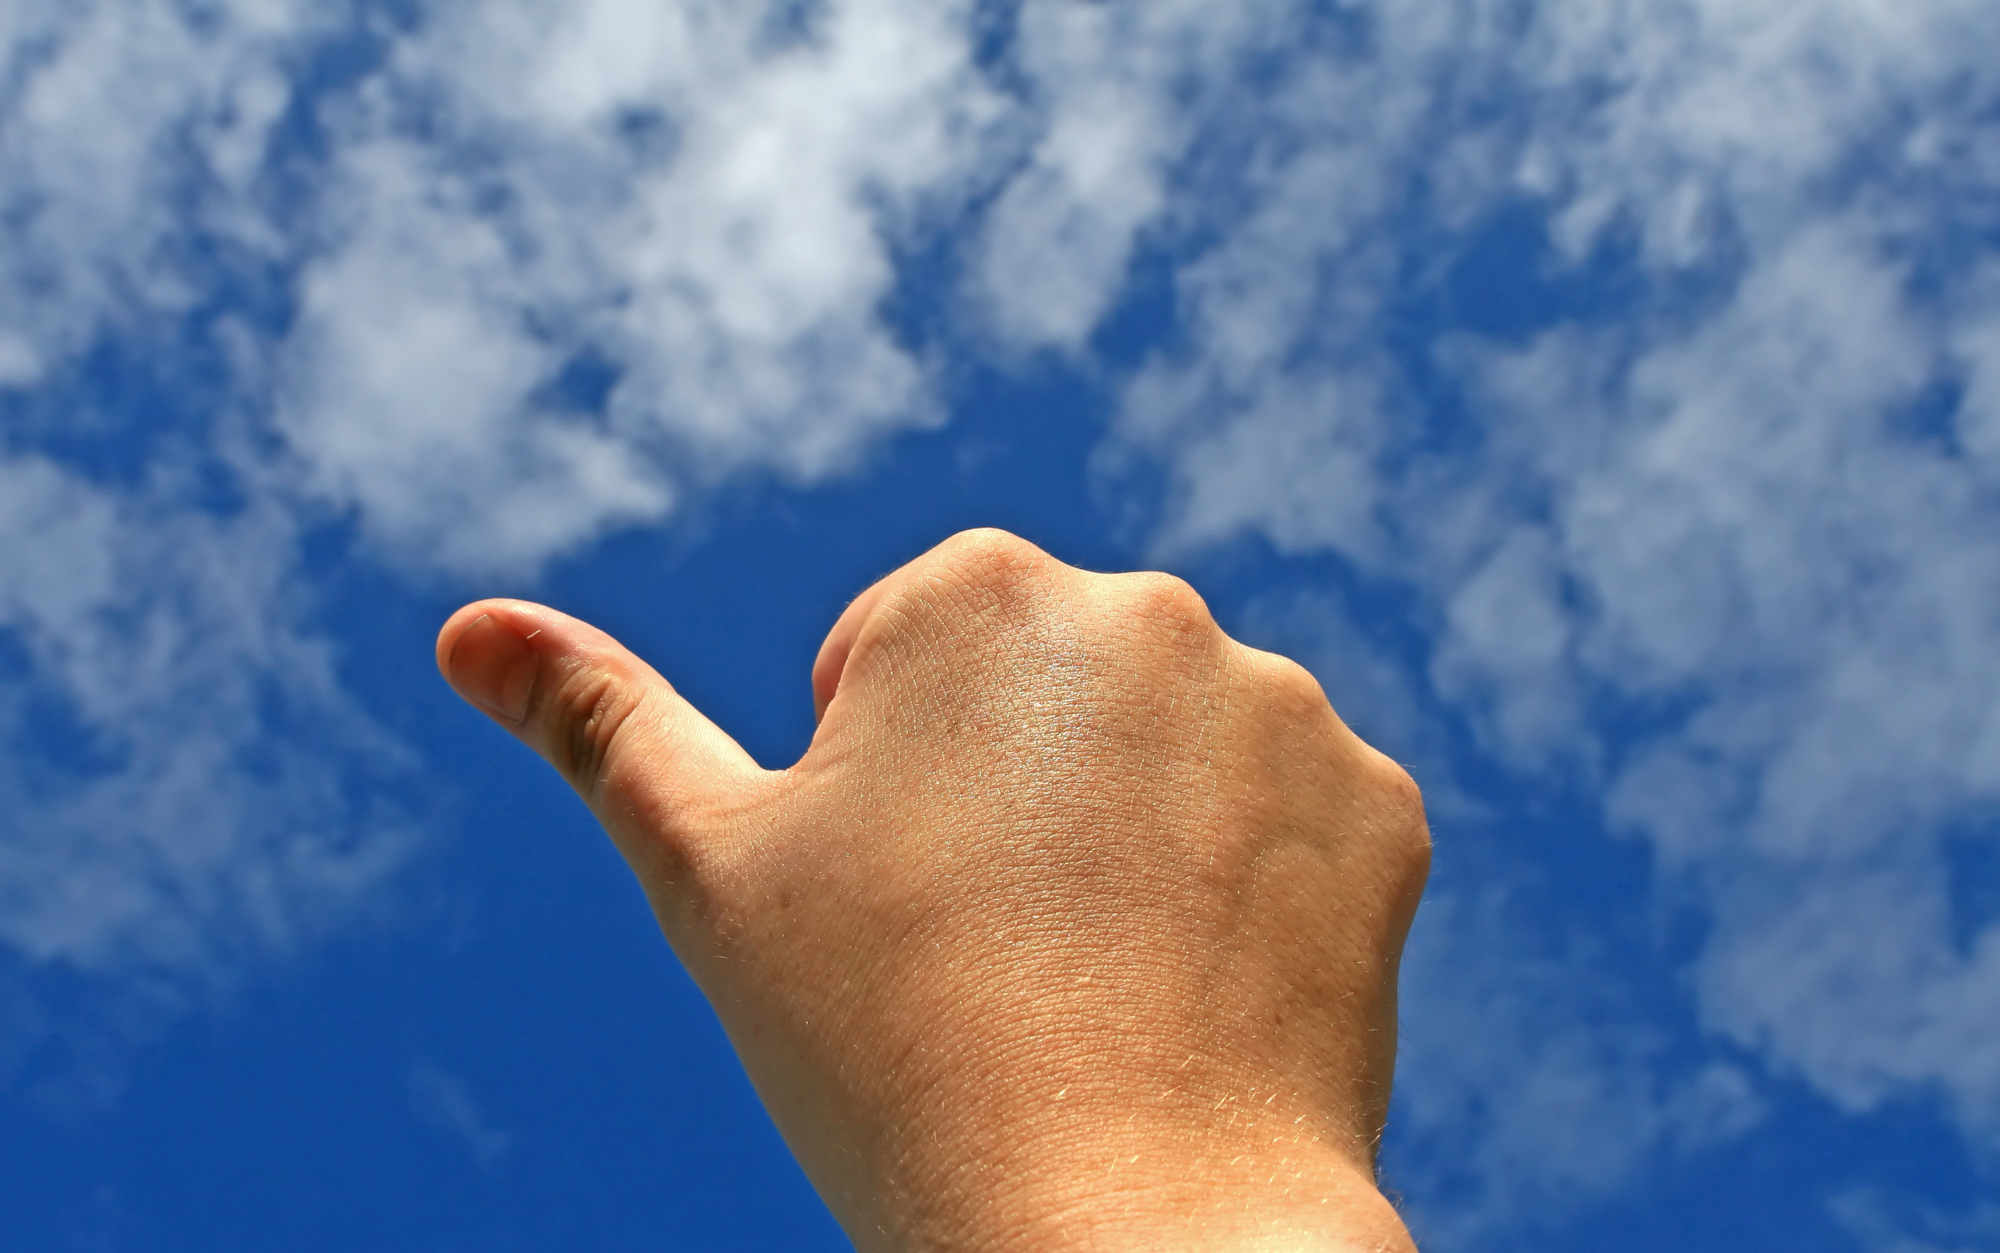
\includegraphics[height=8cm]{\imgGl/thumb-sky-819816-pxh.png}
\end{center}

% This file is part of the Open Source project 'proTironeComputatri'
% (c) 2025 Karsten Reincke (https://github.com/kreincke/proTironeComputatri)
% It is distributed under the terms of the creative commons license
% CC-BY-4.0 (= https://creativecommons.org/licenses/by/4.0/)

\subsection{Thema: Aspekt}

\begin{center}
  \includegraphics[height=8cm]{\imgGl/bird-flower-267994-pxh.png}
\end{center}




Und hier ein Fußnotentest\footcite[vgl.][17]{RlpIt2019a}

\addsec{Bildnachweise}
\begin{itemize}
   \item \includegraphics[height=8pt]{\imgGl/bird-flower-267994-pxh.png} von Andy Morffew. \href{https://pxhere.com/en/photo/267994}{Lizenziert} unter \href{https://creativecommons.org/licenses/by/2.0/}{CC-BY-2.0}. Bereitgestellt auf \href{https://pxhere.com/en/photo/267994}{Pxhere:267994}.
   \item \includegraphics[height=8pt]{\imgGl/bird-flower-267994-pxh.png} von Andy Morffew. \href{https://pxhere.com/en/photo/267994}{Lizenziert} unter \href{https://creativecommons.org/licenses/by/2.0/}{CC-BY-2.0}. Bereitgestellt auf \href{https://pxhere.com/en/photo/267994}{Pxhere:267994}.
   \item \includegraphics[height=8pt]{\imgGl/logo-protirone.png} von Karsten Reincke. \href{https://github.com/kreincke/proTironeComputatri/blob/main/LICENSING.md}{Lizenziert} unter \href{https://github.com/kreincke/proTironeComputatri/blob/main/LICENSING.md}{proTirone-Logo-License}. Bereitgestellt auf \href{https://github.com/kreincke/proTironeComputatri/}{github}. (may only be used as logo for proTirone)
\end{itemize}


\printbibliography
\input{\bibGl/ncl.abbrevs-de.tex}
\input{\bibGl/ncl.journals.tex}
\printnomenclature

\end{document}
